\documentclass[conference]{IEEEtran}
\IEEEoverridecommandlockouts
% The preceding line is only needed to identify funding in the first footnote. If that is unneeded, please comment it out.
\usepackage{cite}
\usepackage{amsmath,amssymb,amsfonts}
\usepackage{algorithmic}
\usepackage{graphicx}
\usepackage{textcomp}
\usepackage{xcolor}
\usepackage{booktabs}
\def\BibTeX{{\rm B\kern-.05em{\sc i\kern-.025em b}\kern-.08em
    T\kern-.1667em\lower.7ex\hbox{E}\kern-.125emX}}
\begin{document}

\title{Mini Project 1\\}

\author{\IEEEauthorblockN{Claire Hattaway}
\IEEEauthorblockA{\textit{och240} \\
\textit{NYU CS-GY 6313 Information Visualization}}
}

\maketitle

\section{Introduction}
For Mini Project 1, we were given a dataset of temperature records that represent global temperature anomalies over the span of 1880 to 2025. After performing data cleaning and standardization, the temperature records were plotted with a diverging palette to color code temperatures that were below the 20\textsuperscript{th}-century mean, and the top 5 warmest years were calculated.

\section{Processing the Data}

\subsection{Data Cleaning}

The first step to this mini project involved data cleaning to transform the date and temperature anomaly data into standard forms. Using the pandas library in Python, I first cast all the dates to a standard datetime format, which required handling a few edge cases separately that pandas was unable to deduce, such as "Mar-19" to March 2019. Next, there were several rows where the temperature anomalies appeared in the date column, while the dates appeared in the temperature column. I was able to swap these values into their correct columns and then perform a few string operations on the temperature column to create a consistent numerical format, including removing "°C" and replacing commas with decimal points. After creating a standard numerical format, I converted the temperature column to a float data type.

\subsection{Outlier Removal}

The next step in this project involved using the IQR method to remove outliers, including the 500error recordings. I used panda's quantile function to find the Q1 and Q3 calculations, then used the following formulae to identify the outliers and replace the outliers with NaN values.
\[IQR=Q3-Q1\]
\[x<Q1-1.5*IQR\quad \text{or} \quad x>Q3+1.5*IQR\]

\subsection{Interpolation and Normalization}

After removing the outliers from the dataset, I then used panda's interpolate function using the method argument to specify a linear interpolation. Once the NaN values were filled using linear interpolation, I then normalized the temperatures using Z-score standardization into a separate column for producing the visual plot. The Z-score standardization was calculated using the following formula.
\[z=\frac{x-\mu}{\sigma}\]

\section{Results}

\subsection{Five Warmest Years}
After the data processing was completed, I could now proceed to finding the top five warmest years and plotting the global temperature anomolies over time. Using panda's group by function, I was able to compute the average temperature for each year, which yielded the results captured in the table below. 

\begin{table}[h]
    \centering
    \begin{tabular}{c c}
        \toprule
        Year & Temperature Anomaly Average (°C) \\
        \midrule
        2024 & 1.74 \\
        2023 & 1.72 \\
        2025 & 1.58 \\
        2016 & 1.55 \\
        2022 & 1.53 \\
        \bottomrule
    \end{tabular}
\end{table}

\subsection{Temperature Anomolies Over Time}\label{AA}
After computing the top five warmest years, the temperature anomalies were plotted over time, using the normalized values. Additionally, the plots were color-coded according to if they were above the 20\textsuperscript{th}-century average. To determine the 20\textsuperscript{th}-century average, I isolated the data between January 1901 and December 2000, based on a search to validate the years contained in the century and computed the mean.\cite{b1}

\begin{figure}[ht]
    \centering
    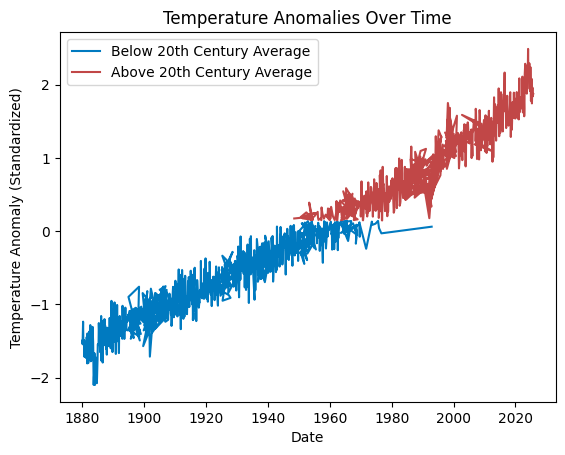
\includegraphics[width=\linewidth]{Mini-Project-Graph.png}
\end{figure}

\begin{thebibliography}{00}
\bibitem{b1}“The 21st Century and the 3rd Millennium.” Astronomical Applications Department, U.S. Navy, aa.usno.navy.mil/faq/millennium. Accessed 11 Feb. 2026. 
\end{thebibliography}

\end{document}
